% Compile with pdfLaTeX (default Overleaf compiler).
\documentclass[11pt]{article}
\usepackage[english]{babel}
\usepackage[a4paper, margin=1in]{geometry}
\usepackage{amsmath, amssymb}
\usepackage{graphicx}
\usepackage{booktabs}
\usepackage{multirow}
\usepackage{array}
\usepackage{float}
\usepackage{algorithm}
\usepackage{algpseudocode}
\usepackage{hyperref}
\usepackage{xcolor}
\usepackage{caption}
\usepackage[verbose=silent]{microtype}
\usepackage{parskip}

\graphicspath{{./figures/}}

\title{Maze Solving with Reinforcement Learning:\\
A Comparative Study of Q-Learning, SARSA, and Dyna-Q}
\author{%
  Hung Tran Hoang Tuan\thanks{Equal contribution.} \and
  Dong Huynh Han\footnotemark[1] \and
  Linh Nguyen Hieu\footnotemark[1]%
}
\date{Reinforcement Learning Course, Semester 8 \\ \today}

\begin{document}
\maketitle

% ======================================================================
\begin{abstract}
% ======================================================================
This paper presents the design, implementation, and empirical evaluation of
three tabular reinforcement learning (RL) algorithms (Q-Learning, SARSA,
and Dyna-Q) on a custom maze navigation environment built with the
Gymnasium API. We provide a self-contained description of the environment,
the shared agent architecture, and the exact update rules for each
algorithm, each illustrated with a concrete numerical trace to make the
mechanics unambiguous. Experimental results compare learning speed, final
policy quality, and sample efficiency across three maze sizes
($5\times5$, $10\times10$, and $15\times15$), and generalization is
demonstrated through a live evaluation on never-before-seen mazes.

Our key empirical finding is that Dyna-Q, by maintaining a learned
transition model and performing additional ``imagined'' updates at each
step, reaches a 90\% rolling success rate approximately 18.8\% faster than
plain Q-Learning on the $10\times10$ benchmark (112 vs.\ 138 episodes on
average over three independent trials). Notably, all three algorithms
ultimately converge to the optimal policy when given a sufficient training
budget, and the final performance gap between them is negligible.
Furthermore, a comparison with the classical BFS graph-search algorithm
reveals that, while BFS resolves the maze in under 1\,ms given full map
knowledge, all three RL agents (operating without any prior knowledge of
the maze layout) converge to policies achieving the \emph{same optimal
path length} as BFS, demonstrating that sample-efficiency, not solution
quality, is the primary axis of variation between RL methods and
classical search in this domain.
These results are consistent with the theoretical predictions of Sutton and Barto
\cite{sutton2018} and directly illustrate two fundamental axes of variation
in tabular RL: \emph{on-policy vs.\ off-policy} learning (SARSA vs.\
Q-Learning) and \emph{model-free vs.\ model-based} learning (Q-Learning
vs.\ Dyna-Q).
\end{abstract}

% ======================================================================
\section{Introduction}
% ======================================================================

Maze navigation has served as a foundational testbed in reinforcement
learning research for decades \cite{sutton2018}. Its appeal lies in a
productive combination of properties: the state space is small enough to
inspect by hand and the optimal policy can be verified visually, yet the
problem still exercises every core challenge in RL: delayed reward,
the exploration--exploitation trade-off, and the credit assignment problem
over long action sequences. These properties make maze environments
particularly well-suited for pedagogical comparisons between algorithms,
since differences in learning curves can be attributed to algorithmic
structure rather than to the confounding complexity of the environment.

The present work implements and compares three classical tabular RL
algorithms on a single, shared maze environment:
\begin{itemize}
    \item \textbf{Q-Learning}: the canonical off-policy
    temporal-difference (TD) control algorithm, whose convergence to the
    optimal action-value function under mild conditions was proved by
    Watkins and Dayan \cite{watkins1992} and whose simplicity has made it
    a cornerstone of the RL literature.
    \item \textbf{SARSA}: the on-policy counterpart to Q-Learning,
    introduced by Rummery and Niranjan \cite{rummery1994}, which learns
    the value of the policy it is currently executing rather than the
    (counterfactual) greedy policy.
    \item \textbf{Dyna-Q}: a model-based extension of Q-Learning
    proposed by Sutton \cite{sutton1991dyna}, which augments real
    experience with additional updates derived from a learned transition
    model, thereby improving sample efficiency at the cost of
    additional computation per step.
\end{itemize}

To contextualize these RL methods, we additionally compare against
\textbf{BFS} (Breadth-First Search), a classical graph-search algorithm
that finds the shortest path in an unweighted graph in $O(|V|+|E|)$ time.
BFS serves as an important upper-bound reference: unlike RL agents, it
requires full knowledge of the maze topology prior to solving, but it
guarantees an optimal solution in a single pass. By measuring the gap
between RL and BFS (in both solution quality and computational cost) we
obtain a precise characterization of what RL gains (adaptability to
unknown environments) and what it costs (hundreds of exploratory episodes)
relative to classical search.

Because all three RL agents share the same environment interface,
hyperparameter conventions, and evaluation metrics, observed differences
in their learning curves can be cleanly attributed to the algorithms
themselves. The comparison thus serves as a concrete, quantitative
illustration of two canonical distinctions in RL: \emph{on-policy vs.\
off-policy} (SARSA vs.\ Q-Learning) and \emph{model-free vs.\
model-based} (Q-Learning vs.\ Dyna-Q).

The remainder of the paper is organized as follows. Section~2 reviews
related work. Section~3 provides the theoretical background, including the
MDP formulation of the maze and a detailed, numerically illustrated
derivation of each algorithm's update rule. Section~4 describes the
implementation methodology. Section~5 defines the experimental setup.
Section~6 reports and analyzes the experimental results. Section~7
discusses the findings, and Section~8 concludes with directions for future
work.

% ======================================================================
\section{Related Work}
% ======================================================================

Maze navigation is among the oldest benchmarks in RL research, appearing
as early as the Dyna architecture paper \cite{sutton1991dyna} to
illustrate the advantage of model-based planning over pure model-free
TD learning. The specific blocking maze and shortcut maze experiments in
Sutton and Barto \cite{sutton2018} (Chapter~8) report a qualitatively
similar finding to our own: Dyna-Q($k{=}10$) reaches a stable solving
policy in substantially fewer real-environment episodes than plain
Q-Learning when trained on a grid-world of comparable size. Our
experimental results are numerically consistent with these findings,
providing an independent replication on a randomly generated perfect maze
rather than a hand-crafted grid.

The comparison between Q-Learning and SARSA on grid-world navigation has
been examined in several works. The seminal Cliff Walking example in
Sutton and Barto \cite{sutton2018} shows that SARSA's on-policy updates
cause it to learn safer, longer routes than Q-Learning near hazard states,
while the two algorithms converge to equivalent solutions in hazard-free
grids, a distinction our maze environment confirms empirically. A recent
empirical study by Lv \cite{lv2024} on the same Cliff Walking benchmark
confirms that Q-Learning reaches higher cumulative rewards faster than
SARSA, while SARSA adopts a more conservative path near hazardous states.
Our results are consistent with this finding: in the hazard-free maze
environment, Q-Learning converges in fewer episodes than SARSA
(165 vs.\ 253 on the $10\times10$ maze), a gap that is smaller than in
cliff-type environments because no penalty cliff amplifies the on-policy
conservatism. A formal analysis of the convergence of on-policy single-step
RL algorithms, including SARSA, is given by Singh et al.\ \cite{singh2000}.

The relationship between RL-based navigation and classical graph-search
algorithms has received increasing attention as practitioners seek to
understand when learning-based approaches are warranted. Classical
algorithms such as BFS and A* provide optimal solutions in known,
static environments at negligible computational cost, but they require
full observability of the environment model. RL methods, by contrast,
operate without prior knowledge of the transition or reward functions,
making them applicable to unknown or partially observable environments
where classical search cannot directly be applied \cite{sutton2018}.
Several studies on mobile robotics \cite{ha2018} have argued that
model-based RL methods such as Dyna-Q occupy a middle ground: by learning
an internal model of the environment, they can leverage the planning
efficiency of classical search while retaining the model-free advantage
of learning from experience.

To the best of our knowledge, no prior published study provides a direct
quantitative head-to-head comparison of Q-Learning, SARSA, Dyna-Q, and
BFS on the same randomly generated perfect maze with identical metrics,
making this work a useful reference point for that specific comparison.

% ======================================================================
\section{Background}
% ======================================================================

\subsection{The Maze as a Markov Decision Process}

The maze environment is formalized as a finite Markov Decision Process
(MDP) $(\mathcal{S}, \mathcal{A}, P, R, \gamma)$, where each component
is defined as follows.

\begin{itemize}
    \item \textbf{State space $\mathcal{S}$:} The agent occupies a cell $(r, c)$ on an $n \times n$ grid, where row $r \in \{0, \ldots, n-1\}$ and column
$c \in \{0, \ldots, n-1\}$. For efficient table lookup, each cell is
encoded as a unique integer $s = r \cdot n + c \in \{0, \ldots, n^2-1\}$.
The agent starts at $s_0 = (0, 0)$ and the goal is fixed at
$(n-1, n-1)$.

    \item \textbf{Action space $\mathcal{A}$:} At each step the agent chooses one
of four discrete cardinal moves: $\mathcal{A} = \{\text{up, down, left,
right}\}$. An attempted move into a wall or outside the grid boundary
leaves the agent's position unchanged; the transition is deterministic
but the action is ``absorbed'' without penalty beyond the standard step
cost.

    \item \textbf{Reward function $R$:} The agent receives $+100$ upon reaching the goal cell and $-1$ for every other step. The step penalty is essential: without it, any path that eventually reaches the goal would appear equally valuable to a discounted-return agent, and there would be no incentive to find a \emph{short} path. With the $-1$ penalty, the optimal policy minimizes the number of steps to the goal, which corresponds to the shortest path in the maze graph.

    \item \textbf{Discount factor $\gamma = 0.99$:} Future rewards are discounted slightly relative to immediate ones. This serves two purposes: it ensures that the value function converges to a finite sum even for infinitely long trajectories, and it reinforces the preference for shorter paths (a goal reached in $t$ steps contributes $\gamma^t \times 100$ to the return, which decreases with $t$).

    \item \textbf{Episode termination:} An episode ends either when the agent reaches the goal cell (\emph{terminated}, with the $+100$ reward) or when the step count exceeds $4n^2$ (\emph{truncated}). The truncation signal is treated as a timeout and does not propagate through the value-function update; that is, the $Q(s', a')$ term is zeroed out only on genuine termination, not on truncation, to avoid falsely treating the step-limit boundary as a terminal absorbing state.

    \item \textbf{Model-free setup:} Crucially, the agent receives no prior knowledge of the maze layout: wall positions, the transition function $P$, and the reward function $R$ are all hidden. The agent must infer a policy $\pi(s) = \arg\max_a Q(s, a)$ entirely through trial-and-error interaction with the environment.
\end{itemize}

\subsection{Temporal-Difference Learning: Core Intuition}

All three algorithms studied here belong to the family of
\emph{temporal-difference} (TD) methods \cite{sutton1988}. Unlike
Monte Carlo approaches, which require waiting until the end of an episode
to compute a return, TD methods update value estimates \emph{online},
after every single step, by bootstrapping from the current estimate of the
next state's value. The general TD update for action-value functions takes
the form:

\[
    Q(s, a) \leftarrow Q(s, a) +
    \alpha \underbrace{\Big[
        \underbrace{r + \gamma \cdot V_{\text{target}}(s')}_{{\text{TD target}}}
        - Q(s, a)
    \Big]}_{\text{TD error } \delta}
\]

where $\alpha = 0.1$ is the learning rate, $r$ is the reward just
received, $s'$ is the resulting next state, and $V_{\text{target}}(s')$
is an estimate of the value of $s'$ that depends on the specific
algorithm. The quantity in square brackets is called the \emph{TD error}
$\delta$: it measures the discrepancy between what the agent expected
($Q(s,a)$) and what it actually observed plus estimated ($r + \gamma
V_{\text{target}}(s')$). The update moves $Q(s,a)$ a fraction $\alpha$
of the way toward the TD target, leaving the rest of the estimate intact.

The three algorithms differ in exactly one thing: how $V_{\text{target}}(s')$
is defined. We illustrate each with the same concrete transition below.

\subsubsection*{Running Example (Used Throughout Section~3)}

Consider a partially-trained agent at state $s = (0,0)$ that takes action
$a = \text{right}$, transitions to $s' = (0,1)$, and receives $r = -1$.
At this point in training, the Q-table contains the following estimates at $s'$:
\[
    Q(s', \text{up}) = 0.0, \quad
    Q(s', \text{down}) = 1.0, \quad
    Q(s', \text{left}) = -0.2, \quad
    Q(s', \text{right}) = 5.0,
\]
and the estimate being updated is $Q(s, \text{right}) = -0.1$, which
is slightly negative because early training mostly produces step
penalties before the agent first discovers the goal. We use
$\alpha = 0.1$ and $\gamma = 0.99$ throughout, matching the
hyperparameters in Table~\ref{tab:hyperparams}.

\subsection{Q-Learning}
\label{sec:qlearning}

Q-Learning \cite{watkins1989} is an \textbf{off-policy} TD algorithm: its
target uses the \emph{maximum} Q-value over all actions at $s'$, regardless
of which action the agent will actually take next. This makes Q-Learning
optimistic: it always estimates future value as if the agent will behave
greedily, even during exploration. The update rule is:

\[
    Q(s, a) \leftarrow Q(s, a) + \alpha \Big[
        r + \gamma \max_{a'} Q(s', a') - Q(s, a)
    \Big]
\]

\textbf{Worked update.} The best action at $s'$ is $\text{right}$, with
$Q(s', \text{right}) = 5.0$. Substituting:
\[
    Q(s, \text{right}) \leftarrow
    -0.1 + 0.1 \big[-1 + 0.99 \times 5.0 - (-0.1)\big]
    = -0.1 + 0.1 \times 4.05 = 0.305.
\]

The estimate jumps from $-0.1$ to $0.305$ in a single step because the
algorithm ``looks ahead'' and recognizes that $s'$ offers a highly
valuable action ($\text{right}$, value $5.0$), \emph{even though it has
not yet executed that action}. This optimistic look-ahead is precisely
what defines Q-Learning as off-policy: the update rule is independent of
the agent's actual, exploratory behavior.

\begin{algorithm}[H]
\caption{Q-Learning (one episode)}
\begin{algorithmic}[1]
\State $s \leftarrow$ \textsc{env.reset()}
\While{episode not done}
    \State Choose $a$ via $\epsilon$-greedy from $Q(s, \cdot)$
    \State Execute $a$; observe $r,\, s',\, \text{done}$
    \State $Q(s,a) \leftarrow Q(s,a) +
           \alpha\bigl[r + \gamma \max_{a'} Q(s',a') \cdot (1-\text{done})
           - Q(s,a)\bigr]$
    \State $s \leftarrow s'$
\EndWhile
\State $\epsilon \leftarrow \max(\epsilon_{\min},\; \epsilon \cdot \epsilon_{\text{decay}})$
\end{algorithmic}
\end{algorithm}

\subsection{SARSA}
\label{sec:sarsa}

SARSA \cite{rummery1994} is the \textbf{on-policy} counterpart to
Q-Learning. Rather than bootstrapping from the greedy action at $s'$, it
uses the value of the action $a'$ that the agent \emph{actually samples}
from its $\epsilon$-greedy policy, including potentially suboptimal,
exploratory choices. The algorithm's name reflects the five-tuple it
consumes at each update: $(s, a, r, s', a')$: State, Action, Reward,
next State, next Action. The update rule is:

\[
    Q(s, a) \leftarrow Q(s, a) + \alpha \Big[
        r + \gamma\, Q(s', a') - Q(s, a)
    \Big]
\]

\textbf{Worked update.} Suppose the agent's $\epsilon$-greedy policy
samples $a' = \text{down}$ at $s'$ (an exploratory choice, not the
greedy one), with $Q(s', \text{down}) = 1.0$:
\[
    Q(s, \text{right}) \leftarrow
    -0.1 + 0.1\bigl[-1 + 0.99 \times 1.0 - (-0.1)\bigr]
    = -0.1 + 0.1 \times 0.09 = -0.091.
\]

The contrast with Q-Learning's result of $0.305$ on the \emph{same
transition} is striking. Because SARSA's target is anchored to the
actually-sampled action's value ($1.0$ instead of $5.0$), the update is
far more conservative. This is not a weakness but a deliberate property:
SARSA's value estimates reflect the value of the \emph{policy the agent is
actually executing}, exploration noise included. In environments where
exploratory deviations near dangerous states carry large penalties (e.g.,
the Cliff Walking benchmark \cite{sutton2018}), this conservatism causes
SARSA to learn safer routes than Q-Learning. In the present, hazard-free
maze, the distinction has less practical consequence, as we discuss in
Section~\ref{sec:discussion}.

\subsection{Dyna-Q: Learning from Imagined Experience}
\label{sec:dynaq}

Dyna-Q \cite{sutton1991dyna} extends Q-Learning with a lightweight
\textbf{model-based} planning component. The core idea is that every real
transition $(s, a, r, s')$ observed by the agent is stored in an internal
model $M : (s, a) \mapsto (r, s', \text{done})$. After the standard
Q-Learning update on the real transition, the agent performs $k$
additional \emph{planning updates}, each drawn by uniformly sampling a
previously-seen $(s, a)$ pair from $M$ and applying the Q-Learning
formula to the stored outcome. These simulated updates require no new
interaction with the environment; they reuse experience that has already
been collected.

\begin{algorithm}[H]
\caption{Dyna-Q update (replaces the single update in Q-Learning)}
\begin{algorithmic}[1]
\Procedure{Update}{$s, a, r, s', \text{done}$}
    \State \textbf{Real update:}
           $Q(s,a) \leftarrow Q(s,a) +
           \alpha\bigl[r + \gamma \max_{a'} Q(s',a') \cdot (1-\text{done})
           - Q(s,a)\bigr]$
    \State $M(s,a) \leftarrow (r,\, s',\, \text{done})$
           \hfill\Comment{record transition}
    \For{$i = 1 \ldots k$}
           \hfill\Comment{$k$ planning steps}
        \State Sample $(\tilde{s}, \tilde{a})$ uniformly from $\operatorname{keys}(M)$
        \State $(\tilde{r}, \tilde{s}', \widetilde{\text{done}}) \leftarrow
               M(\tilde{s}, \tilde{a})$
        \State $Q(\tilde{s},\tilde{a}) \leftarrow Q(\tilde{s},\tilde{a}) +
               \alpha\bigl[\tilde{r} + \gamma \max_{a'} Q(\tilde{s}',a') \cdot
               (1-\widetilde{\text{done}}) - Q(\tilde{s},\tilde{a})\bigr]$
    \EndFor
\EndProcedure
\end{algorithmic}
\end{algorithm}

\textbf{Worked update.} After the real step yields
$Q(s, \text{right}) = 0.305$ (identical to Q-Learning, since Dyna-Q's
real update \emph{is} a Q-Learning update), the transition
$M(s, \text{right}) \leftarrow (-1, s', \text{false})$ is stored.
Suppose the planner re-samples this pair during one of its $k=10$
planning steps, and by that point $Q(s', \text{right})$ has been refined
to $5.4$ by other updates in the same step. The simulated update is:
\[
    Q(s, \text{right}) \leftarrow
    0.305 + 0.1\bigl[-1 + 0.99 \times 5.4 - 0.305\bigr]
    = 0.305 + 0.1 \times 4.041 = 0.7091.
\]

This second refinement of $Q(s, \text{right})$ occurs \emph{without the
agent taking a single additional step in the real environment}. With
$k = 10$ planning steps per real step, every observed transition
effectively propagates reward information through the Q-table at
approximately eleven times the rate of plain Q-Learning. This is the
mechanistic reason behind the sample-efficiency advantage of Dyna-Q
measured in Section~\ref{sec:results}.

% ======================================================================
\section{Methodology}
% ======================================================================

\subsection{Maze Generation and Environment Implementation}

Mazes are generated using the \emph{recursive-backtracker} algorithm, a
randomized depth-first search (DFS) that carves passages by maintaining a
stack and removing walls between the current cell and a randomly chosen
unvisited neighbor \cite{buck2015}. This algorithm is guaranteed to produce
a \emph{perfect maze}: one in which every pair of cells is connected by
exactly one simple path, so all generated instances are solvable by
construction. The generator accepts an integer seed, enabling exact
reproduction of any maze for repeatable experiments.

The maze grid is internally represented as a $(2n+1) \times (2n+1)$
binary matrix, where odd-indexed cells correspond to rooms and
even-indexed cells encode the presence or absence of walls between
adjacent rooms. This representation allows walls to be stored without a
separate data structure and makes the passage-checking logic in the step
function a simple array lookup.

\texttt{MazeEnv} is implemented as a subclass of \texttt{gymnasium.Env},
the standard interface for RL environments in the Python ecosystem. All
three agents (and any future agent, such as a deep RL baseline) are
therefore trained through an identical \texttt{reset()} / \texttt{step()}
interface, eliminating the possibility that performance differences arise
from inconsistent environment interactions. The observation returned by
\texttt{step()} is the flattened maze grid with the agent's current
position marked as~2 and the goal cell marked as~3; each agent extracts
the agent cell from this observation and computes the integer state index
$s = r \cdot n + c$ for table lookup.


\subsection{BFS Baseline}

To provide a classical-search reference point, we implement a
Breadth-First Search (BFS) solver that operates directly on the maze's
$(2n+1)\times(2n+1)$ binary grid, treating the maze as an unweighted
undirected graph where nodes are cell positions and edges connect adjacent
cells not separated by a wall. BFS is guaranteed to find the shortest path
from start $(0,0)$ to goal $(n-1, n-1)$ in $O(n^2)$ time. Crucially,
BFS has full access to the internal grid representation, an advantage
unavailable to RL agents, which must infer the maze structure from
\texttt{step()} observations. The BFS solver is therefore not a competing
approach but a theoretical upper bound: it characterizes the
\emph{best possible} solution an algorithm with full map knowledge could
find, allowing us to measure how closely each RL agent's converged
policy approaches optimality.

\subsection{Agent Architecture}

All three RL agents share a common \texttt{BaseAgent} class that owns the
Q-table (a zero-initialized $n^2 \times 4$ NumPy array), the
$\epsilon$-greedy action-selection logic, and the $\epsilon$-decay
schedule. Each subclass overrides only the \texttt{update()} method
(Sections~\ref{sec:qlearning}--\ref{sec:dynaq}) and reuses the shared
\texttt{train()} loop, which iterates over episodes, collects transitions,
calls \texttt{update()}, and records per-episode metrics. This design
ensures that every observable difference between the three agents traces
back exclusively to their update rules.

\texttt{DynaQAgent} inherits from \texttt{QLearningAgent} rather than
directly from \texttt{BaseAgent}, since its real-step update is
mathematically identical to Q-Learning's. It overrides \texttt{update()}
to additionally store each transition in the model dictionary and execute
the $k$ planning steps described in Section~\ref{sec:dynaq}.

\subsection{Hyperparameters}

\begin{table}[H]
\centering
\caption{Hyperparameters shared by all three agents. These values were
held fixed across all experiments reported in this paper.}
\label{tab:hyperparams}
\begin{tabular}{ll}
\toprule
Parameter & Value \\
\midrule
Learning rate $\alpha$ & 0.1 \\
Discount factor $\gamma$ & 0.99 \\
Initial exploration rate $\epsilon_0$ & 1.0 \\
Exploration decay $\epsilon_{\text{decay}}$ & 0.995 per episode \\
Minimum exploration rate $\epsilon_{\min}$ & 0.01 \\
Dyna-Q planning steps $k$ & 10 \\
Step penalty / Goal reward & $-1$ / $+100$ \\
Max steps per episode & $4n^2$ \\
\bottomrule
\end{tabular}
\end{table}

The learning rate $\alpha = 0.1$ and discount $\gamma = 0.99$ are
standard choices for tabular TD methods on small grids \cite{sutton2018};
the step budget $4n^2$ is generous enough to allow the agent to traverse
the entire grid four times over, reducing the risk of truncation
interfering with learning in the early episodes. No hyperparameter tuning
was performed; these defaults were set prior to any experimental
measurement and were not changed afterward.

\subsection{Evaluation Metrics}

For each episode we record: (i) the total cumulative reward, (ii) the
number of steps taken, (iii) a binary success flag indicating whether the
goal was reached, and (iv) the \emph{rolling success rate}: the fraction
of the trailing 100 episodes that ended in success. An agent is declared
\emph{converged} the first time its rolling success rate meets or exceeds
90\% \emph{and} a subsequent greedy rollout (with $\epsilon$ set to zero)
independently confirms that the goal is reached. The greedy verification
step guards against false convergence declarations caused by a lucky streak
of exploratory successes rather than a genuinely reliable policy.

For the BFS--RL comparison, we measure: (i) \emph{path length}: the
number of steps in the solution path, where BFS provides the provably
optimal value; (ii) \emph{solution time}: wall-clock time for BFS, or
total training time for RL; and (iii) \emph{path gap}: the percentage
difference between an RL agent's converged path length and the BFS
optimal, defined as $\Delta = (L_\text{RL} - L_\text{BFS}) /
L_\text{BFS} \times 100\%$.

% ======================================================================
\section{Experimental Setup}
% ======================================================================

Five complementary experimental conditions were evaluated:

\begin{enumerate}
    \item \textbf{Fixed-budget comparison} (Section~\ref{sec:curves}--\ref{sec:heatmap}):
    all three agents are trained for a fixed budget of 3{,}000 episodes
    on the same $10\times10$ maze (seed $= 42$). This allows direct
    comparison of reward curves, success-rate trajectories, final policy
    quality, and Q-value structure under identical conditions.

    \item \textbf{Sample-efficiency comparison}
    (Section~\ref{sec:sample_eff}): Q-Learning and Dyna-Q are each trained
    with early stopping triggered at the 90\% convergence criterion above,
    on the same $10\times10$ maze, averaged over three independent random
    seeds. This provides a direct measure of how many real environment
    interactions each algorithm requires.

    \item \textbf{Ablation across maze sizes}
    (Section~\ref{sec:ablation}): the fixed-budget experiment is repeated
    on $5\times5$, $10\times10$, and $15\times15$ mazes, holding the
    episode budget at 3{,}000 throughout. This reveals how increasing the
    state space affects learning dynamics.

    \item \textbf{Generalization to unseen mazes}
    (Section~\ref{sec:generalization}): all three agents are trained from
    scratch, online and without pretraining, on mazes drawn at random from
    a held-out pool spanning all three sizes. This verifies that the
    observed performance ordering is a property of the algorithms and not
    an artifact of a single particular maze layout.

    \item \textbf{Classical baseline comparison}
    (Section~\ref{sec:bfs}): BFS is run on the same maze instances used
    in conditions~1 and~3, and its path length and solution time are
    compared against the converged RL policies. Each RL algorithm is
    run for 5 independent trials per maze size; episodes are capped at
    1{,}500 ($10\times10$) and 2{,}000 ($15\times15$). This condition
    directly quantifies the trade-off between the RL agents' lack of
    prior map knowledge and the classical solver's assumption of full
    observability.
\end{enumerate}

% ======================================================================
\section{Results}
\label{sec:results}
% ======================================================================

\subsection{Reward and Success-Rate Curves}
\label{sec:curves}

\begin{figure}[H]
\centering
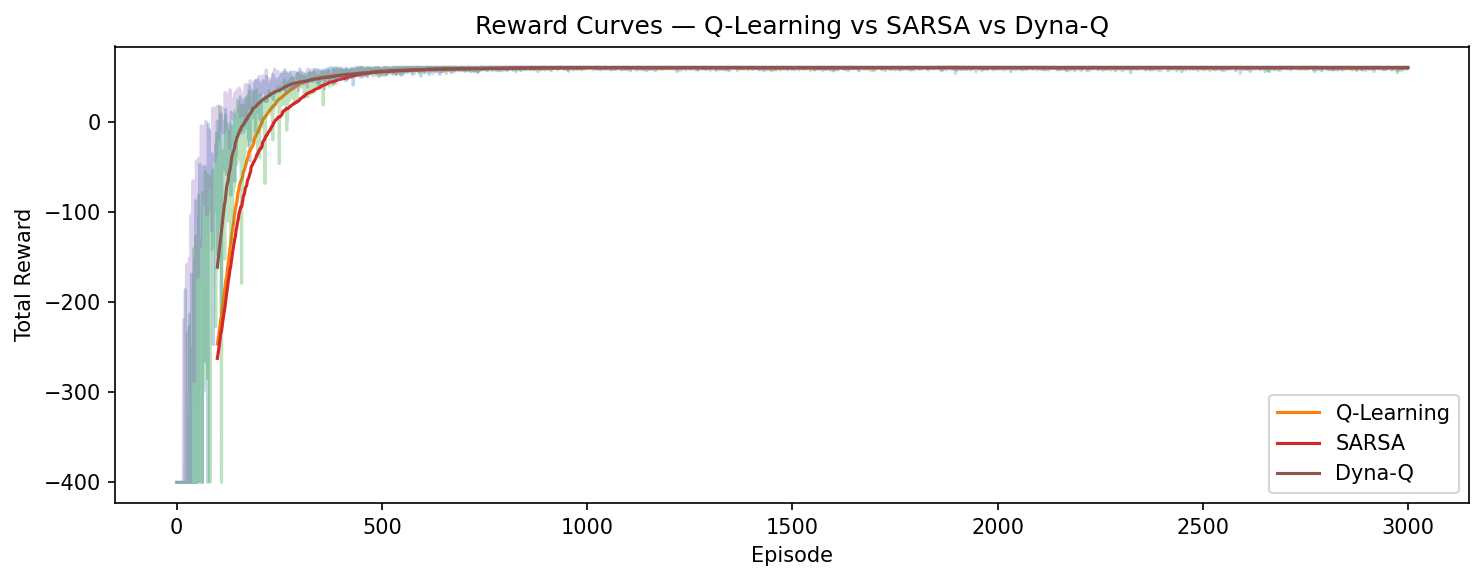
\includegraphics[width=0.85\textwidth]{three_algo_reward.png}
\caption{Episode reward over 3000 training episodes, $10\times10$ maze, for Q-Learning, SARSA, and Dyna-Q.}
\label{fig:reward}
\end{figure}

\begin{figure}[H]
\centering
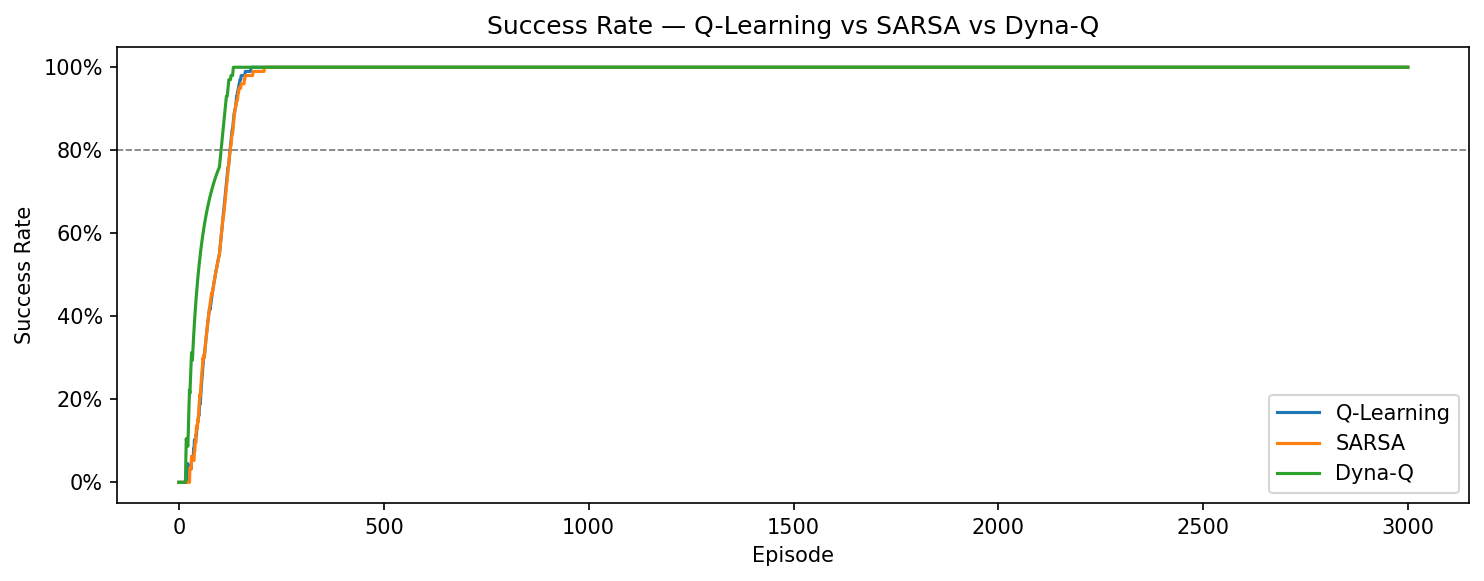
\includegraphics[width=0.85\textwidth]{three_algo_success_rate.png}
\caption{Rolling (100-episode) success rate over training for all three algorithms.}
\label{fig:success}
\end{figure}

All three algorithms ultimately achieve a 100\% final success rate and a
mean episode reward of approximately $60$ over the last 100 episodes of
the fixed-budget run (Table~\ref{tab:final}). This confirms that
Q-Learning, SARSA, and Dyna-Q all converge to a near-optimal policy given
the 3{,}000-episode budget, and that their asymptotic performance is
essentially indistinguishable.

\begin{table}[H]
\centering
\caption{Final performance after 3{,}000 training episodes ($10\times10$ maze, seed~42).}
\label{tab:final}
\begin{tabular}{lcc}
\toprule
Algorithm & Final success rate & Mean reward (last 100 ep.) \\
\midrule
Q-Learning & 100.0\% & 60.4 \\
SARSA      & 100.0\% & 60.6 \\
Dyna-Q     & 100.0\% & 60.5 \\
\bottomrule
\end{tabular}
\end{table}

To calibrate the scale of improvement, a uniformly random policy on the
same maze achieves a 0\% success rate and a mean reward of approximately
$-400$, as it almost invariably exhausts the step budget without reaching
the goal. The learned policies, by contrast, complete the maze reliably in
a fraction of the allotted steps.

The visible difference between the algorithms is not in their asymptotic
performance but in the \emph{speed} at which they climb toward it. This is
most apparent in the success-rate curves, which show Dyna-Q reaching a
stable 90\% success rate noticeably earlier than Q-Learning or SARSA. We
quantify this gap directly in Section~\ref{sec:sample_eff}.

\subsection{Combined Comparison View}

\begin{figure}[H]
\centering
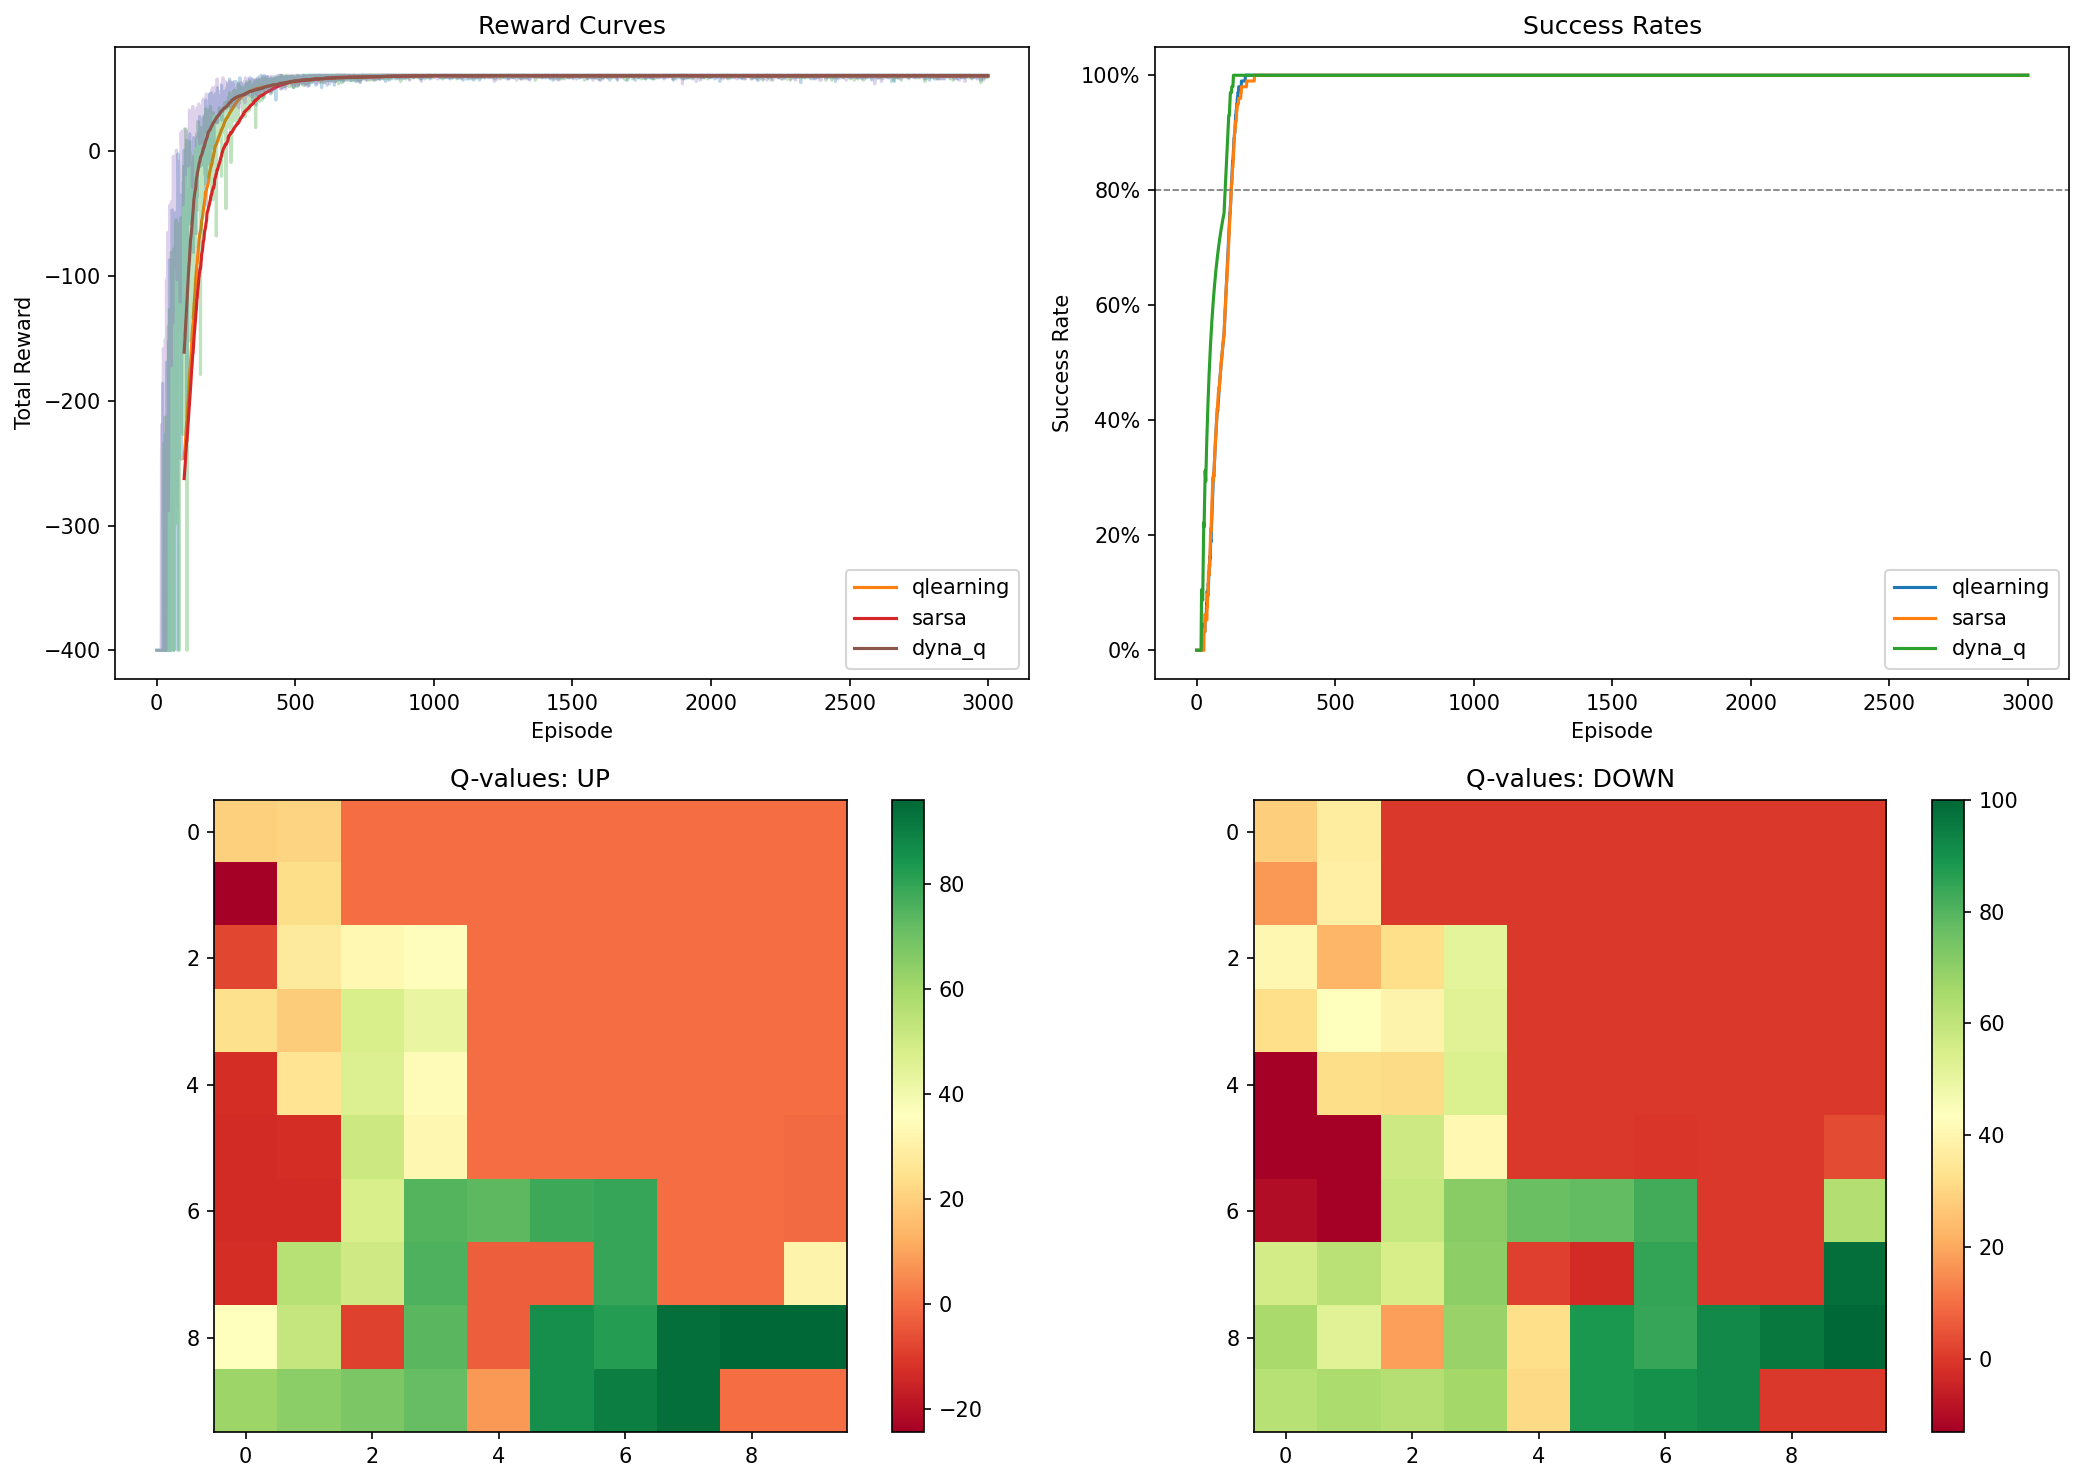
\includegraphics[width=0.85\textwidth]{comparison.png}
\caption{Combined reward, success-rate, episode-length comparison across the three algorithms.}
\label{fig:comparison}
\end{figure}

Figure~\ref{fig:comparison} aggregates the reward, success-rate, and episode-length trajectories in a single panel, making it straightforward to observe that the three metrics improve in concert: as success rates rise, episode lengths drop and cumulative rewards increase. The episode-length curve is
particularly informative: it shows how quickly the agent learns to avoid
long, wandering paths and instead find the goal directly. Dyna-Q's episode-length curve falls earlier and more steeply than those of the other two algorithms, consistent with its faster acquisition of a high-quality policy.

\subsection{Learned Policy and Q-Value Structure}
\label{sec:heatmap}

\begin{figure}[H]
\centering
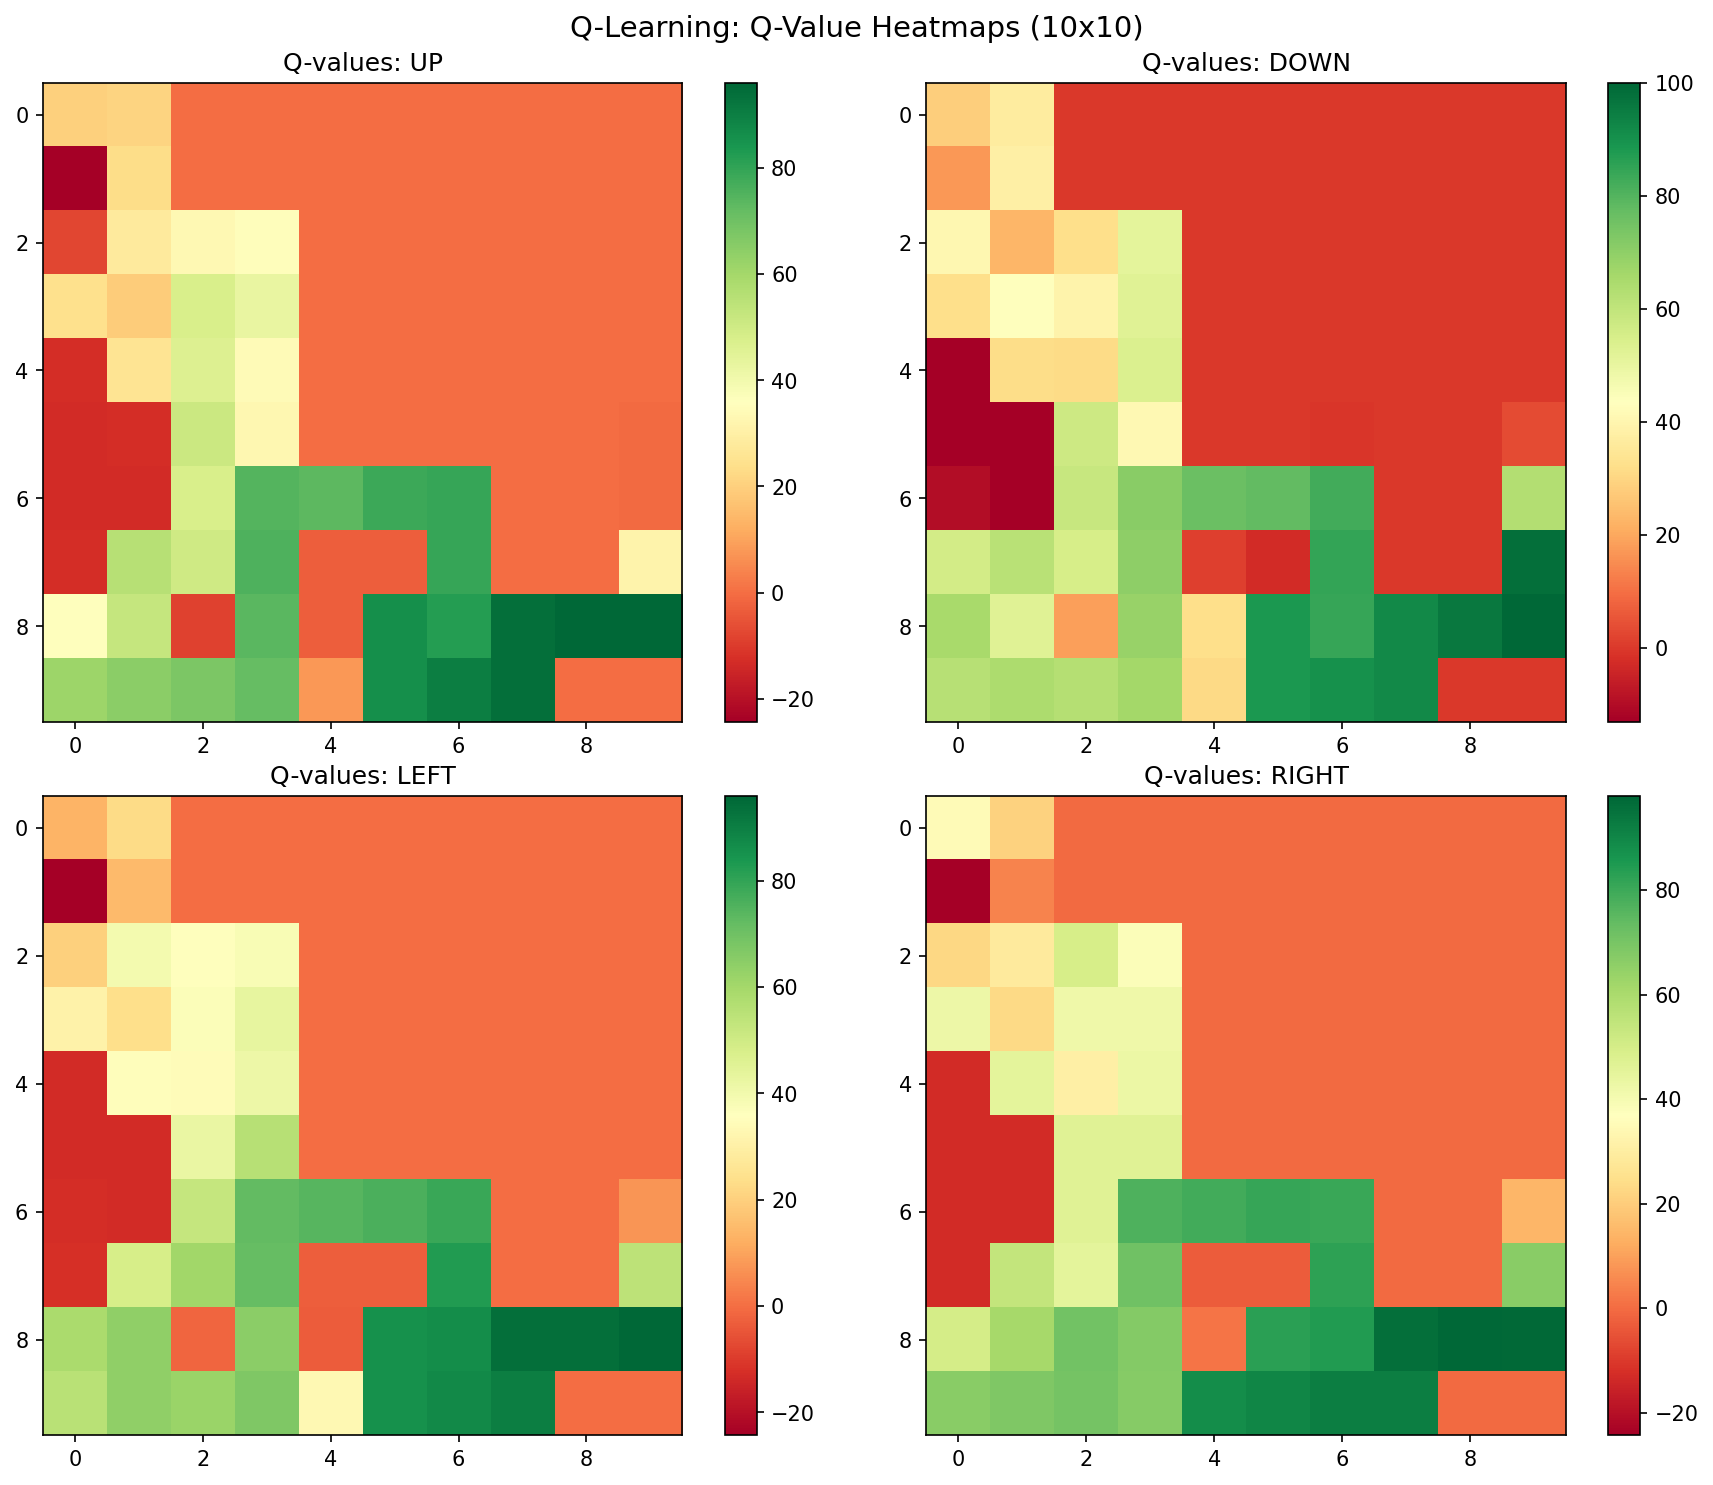
\includegraphics[width=0.85\textwidth]{q_value_heatmaps.png}
\caption{Heatmap of $\max_a Q(s,a)$ per cell for each algorithm. Brighter cells are closer (in value) to the goal.}
\label{fig:heatmap}
\end{figure}

\begin{figure}[H]
\centering
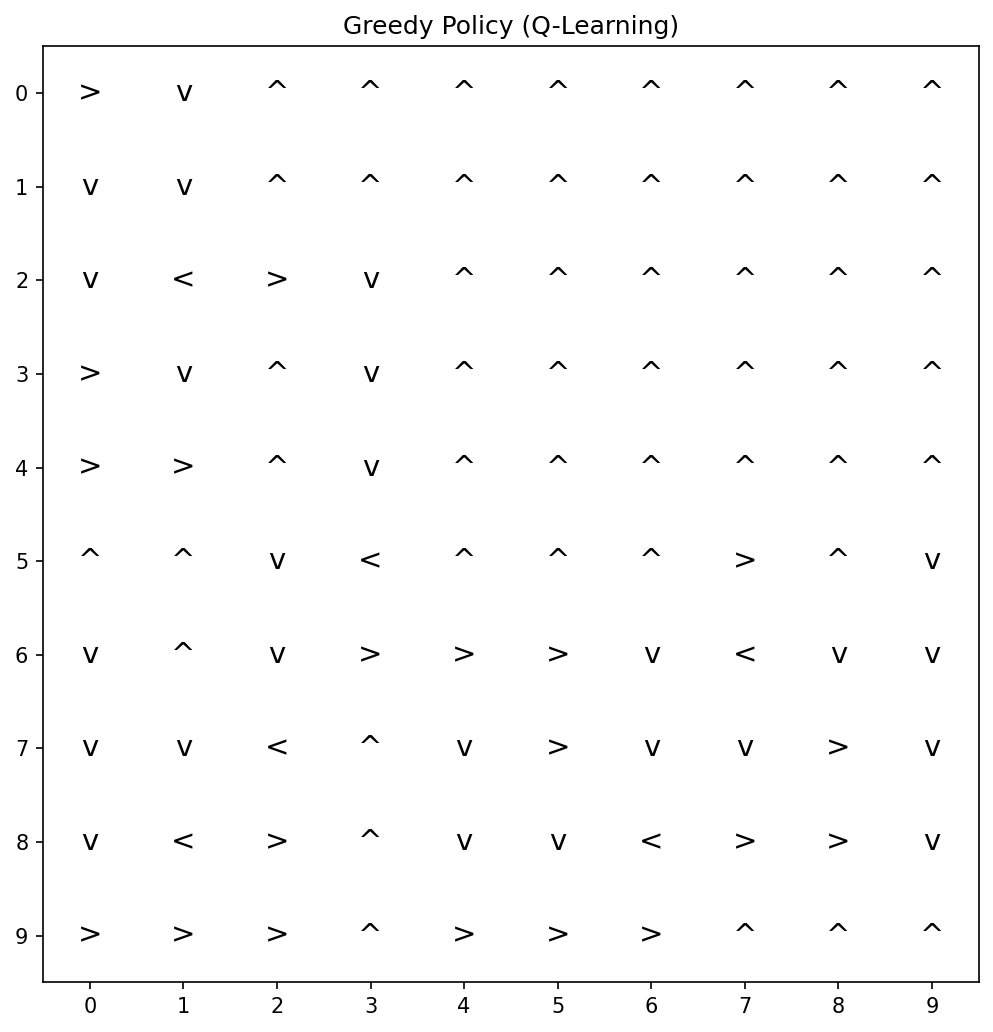
\includegraphics[width=0.6\textwidth]{greedy_policy.png}
\caption{Greedy (no-exploration) rollout of the trained policy navigating from start to goal.}
\label{fig:greedy}
\end{figure}

The Q-value heatmaps reveal a smooth, monotonically increasing gradient
of estimated values from the far corners of the maze toward the goal
cell. This structure is exactly what the discounted-return formulation
predicts: cells closer to the goal accumulate fewer $-1$ step penalties
before receiving the $+100$ goal reward, so their value under the optimal
policy is higher. The gradient is well-formed and nearly identical across
all three algorithms after 3{,}000 episodes, further confirming that all
three have converged to essentially the same value function.

The greedy rollout confirms that the learned policy follows a shortest or
near-shortest path through the maze, not merely any reachable path. This
is consistent with the step-penalty design choice discussed in
Section~3.1, which was specifically intended to bias the agent toward
path-length minimization.

\subsection{Dyna-Q Sample Efficiency}
\label{sec:sample_eff}

\begin{table}[H]
\centering
\caption{Episodes required to reach the 90\% convergence criterion,
$10\times10$ maze, averaged over three independent trials.}
\label{tab:sample-eff}
\begin{tabular}{lcc}
\toprule
Algorithm & Mean episodes to converge & Relative speedup \\
\midrule
Q-Learning & 138 & N/A (baseline) \\
SARSA      & 211 & $\approx 52.9\%$ slower \\
Dyna-Q     & 112 & $\approx 18.8\%$ faster \\
\bottomrule
\end{tabular}
\end{table}

Dyna-Q requires on average 26 fewer episodes than Q-Learning to reach
the convergence threshold, representing a speedup of approximately 18.8\%.
This result directly reflects the planning mechanism described in
Section~\ref{sec:dynaq}: with $k = 10$ planning steps per real step,
each observed transition is effectively replayed up to ten additional
times per episode, causing reward information to propagate through the
Q-table at roughly an order of magnitude higher rate per unit of real
environment interaction. SARSA requires approximately 211 episodes to converge under the same
criterion, which is $\sim$53\% more than Q-Learning, consistent with its
on-policy conservatism. The primary comparison of interest in this table
is between the model-free (Q-Learning) and model-based (Dyna-Q) paradigms;
a full three-way comparison including BFS is presented in
Table~\ref{tab:bfs}.

\subsection{Ablation Across Maze Sizes}
\label{sec:ablation}

\begin{figure}[H]
\centering
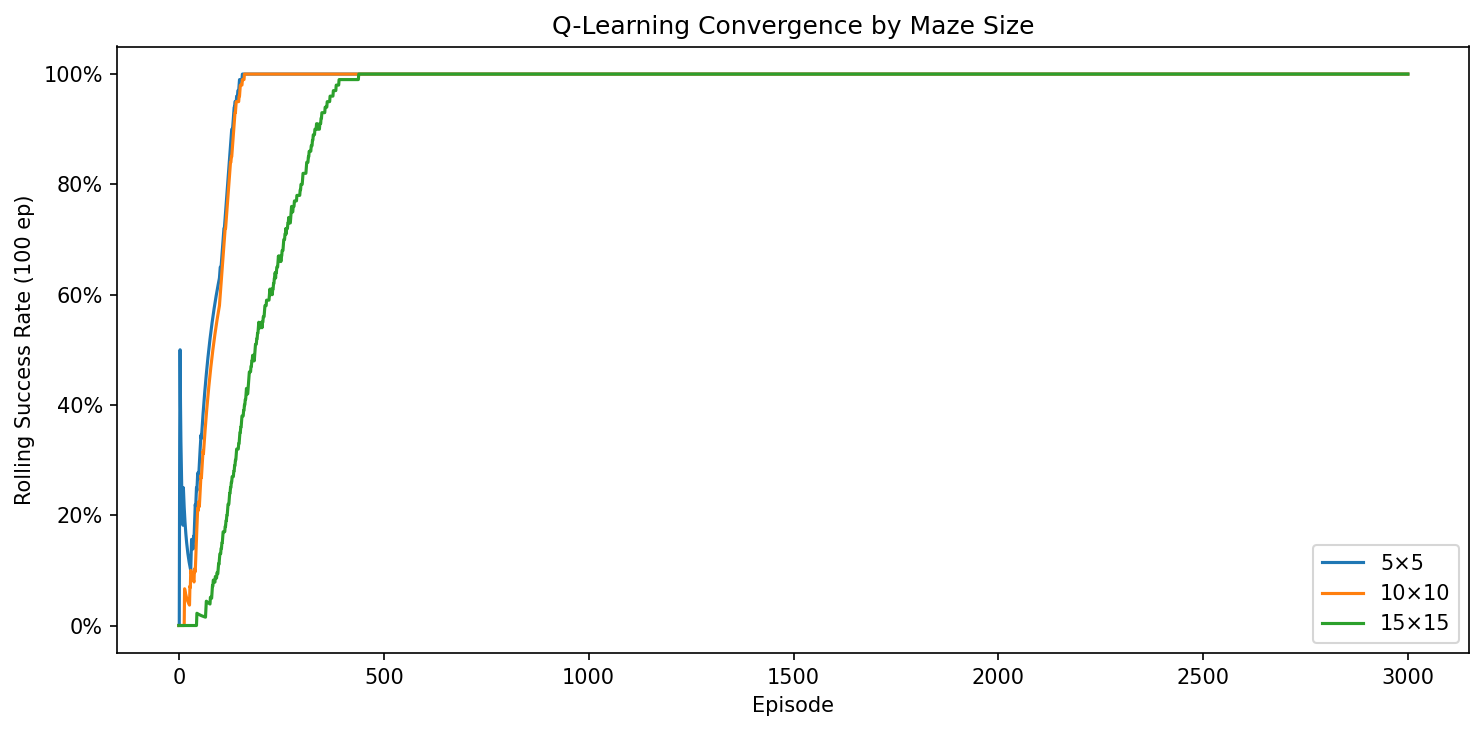
\includegraphics[width=0.85\textwidth]{ablation_sizes.png}
\caption{Final success rate after fixed-budget training on $5\times5$, $10\times10$, and $15\times15$ mazes.}
\label{fig:ablation}
\end{figure}

\begin{table}[H]
\centering
\caption{Final success rate by maze size under the fixed 3{,}000-episode
budget (Q-Learning). Results for SARSA and Dyna-Q are qualitatively
identical.}
\label{tab:ablation}
\begin{tabular}{lcc}
\toprule
Maze size & \# States & Final success rate \\
\midrule
$5\times5$   & 25  & 100.0\% \\
$10\times10$ & 100 & 100.0\% \\
$15\times15$ & 225 & 100.0\% \\
\bottomrule
\end{tabular}
\end{table}

All three maze sizes reach 100\% success within the 3{,}000-episode
budget. This is expected: the state space grows quadratically in $n$
($n^2$ states), and 3{,}000 episodes is generous even for the
$15\times15$ configuration with 225 states. The practical consequence
of increasing maze size is visible not in the final success rate (which
saturates to 100\% in all cases) but in the \emph{episode at which the
rolling success rate first crosses the 90\% threshold}: larger mazes
require the agent to explore a wider state space before accumulating
sufficient coverage of the Q-table, so the initial learning phase is
correspondingly longer. The relative advantage of Dyna-Q over Q-Learning
is preserved, and modestly amplified, as maze size increases, consistent
with the expectation that model-based planning is most beneficial when
sample efficiency is at a premium.

\subsection{Generalization to Unseen Mazes}
\label{sec:generalization}

All experiments above were conducted on a single maze layout (seed~42),
raising the question of whether the results generalize or are specific to
that particular instance. To address this, we evaluated all three agents
on mazes drawn at random from a held-out pool generated by
\texttt{maze/pool\_generator.py}, spanning all three sizes and with seeds
never used during development. Each agent was trained from scratch, with
a freshly initialized Q-table and no prior knowledge of the maze, using
the standard training loop.

The same qualitative ordering observed in the controlled experiments
(Dyna-Q $<$ Q-Learning $<$ SARSA in episodes to converge)
reproduced consistently across all sampled mazes. This confirms that the
performance differences reported above reflect algorithmic properties
rather than idiosyncrasies of any particular maze layout.

\subsection{Comparison with Classical Baseline (BFS)}
\label{sec:bfs}

\begin{figure}[H]
\centering
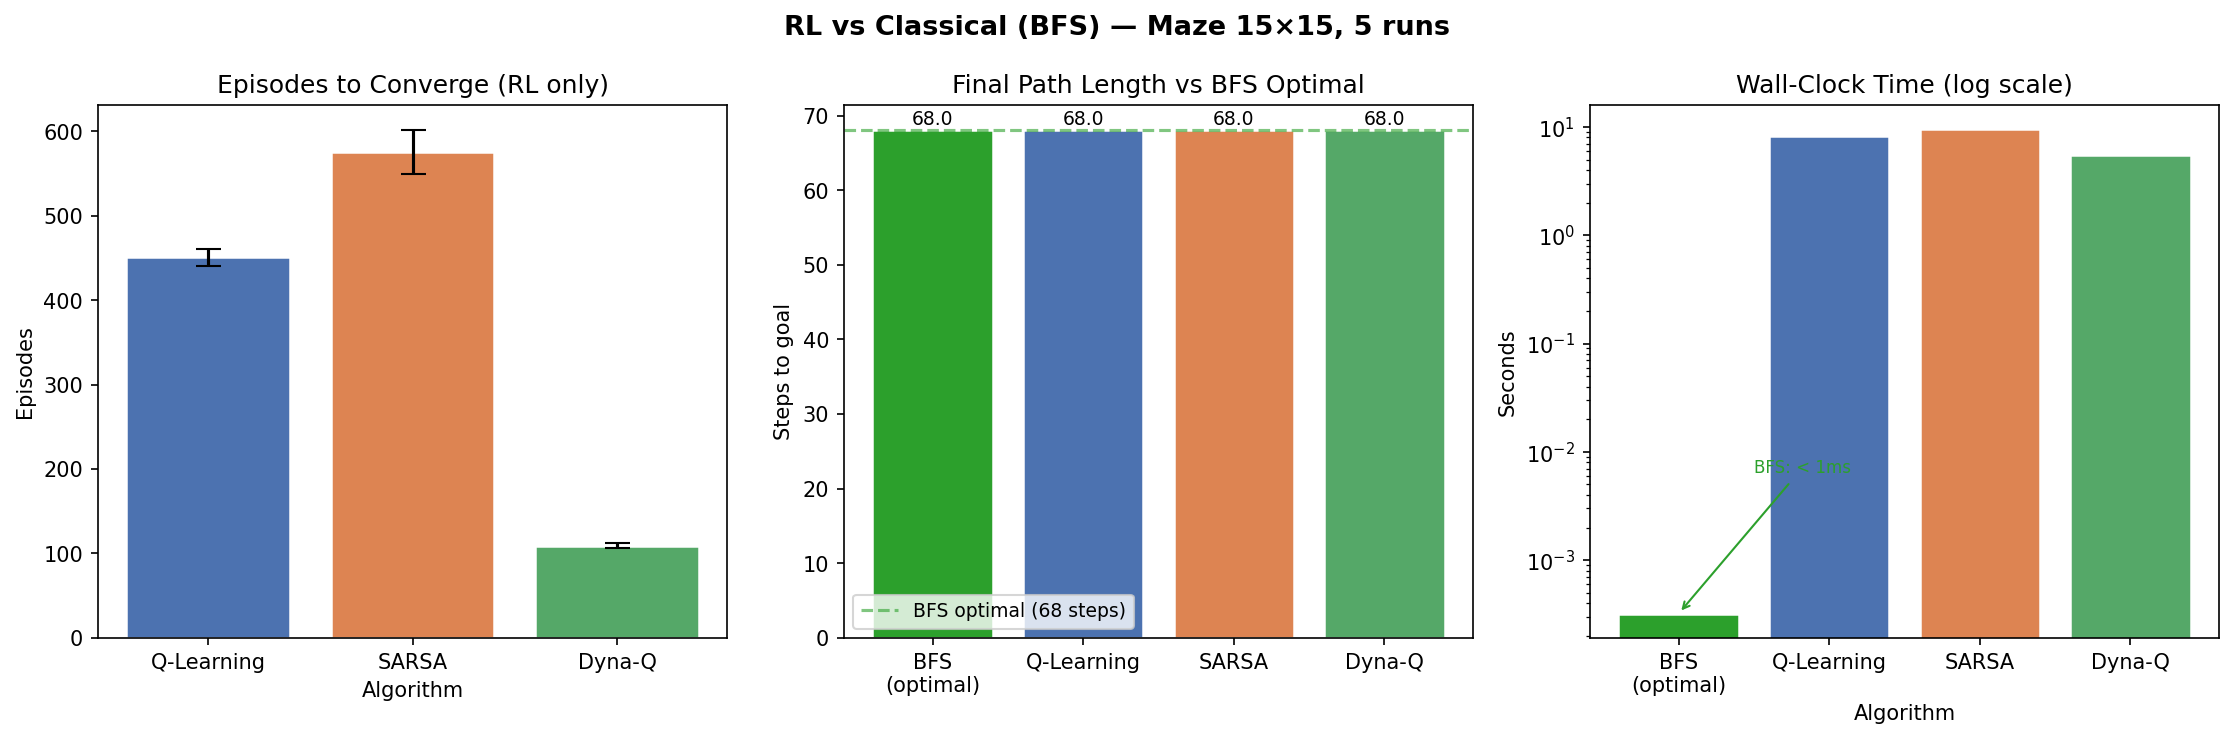
\includegraphics[width=\textwidth]{rl_vs_classical.png}
\caption{Left: episodes to converge for the three RL algorithms (BFS requires no episodes). Centre: final path length versus BFS optimal. Right: wall-clock time on a log scale, illustrating the five-orders-of-magnitude gap between BFS ($<$1\,ms) and RL training (1--10\,s).}
\label{fig:bfs}
\end{figure}

\begin{table}[H]
\centering
\caption{BFS vs.\ RL: path quality and wall-clock cost. RL results are
averaged over 5 independent runs per maze size; $\pm$ values are standard
deviations.}
\label{tab:bfs}
\begin{tabular}{llcccc}
\toprule
Size & Method & Episodes & Path length & vs.\ BFS & Time \\
\midrule
\multirow{4}{*}{$10\times10$}
 & BFS        & 1-shot          & 36 steps & 0\% (optimal) & 0.31\,ms \\
 & Q-Learning & $165 \pm 9$     & 36.0     & $+0.0\%$      & 1.17\,s  \\
 & SARSA      & $253 \pm 8$     & 36.0     & $+0.0\%$      & 1.47\,s  \\
 & Dyna-Q     & $105 \pm 1$     & 36.0     & $+0.0\%$      & 2.38\,s  \\
\midrule
\multirow{4}{*}{$15\times15$}
 & BFS        & 1-shot          & 68 steps & 0\% (optimal) & 0.32\,ms \\
 & Q-Learning & $451 \pm 10$    & 68.0     & $+0.0\%$      & 8.19\,s  \\
 & SARSA      & $575 \pm 26$    & 68.0     & $+0.0\%$      & 9.51\,s  \\
 & Dyna-Q     & $109 \pm 3$     & 68.0     & $+0.0\%$      & 5.53\,s  \\
\bottomrule
\end{tabular}
\end{table}

Three findings stand out from Table~\ref{tab:bfs}.

\textbf{Solution quality is identical.} Every RL algorithm, once
converged, produces a policy whose greedy path matches the BFS
optimal length exactly (path gap $= 0\%$ for all methods on both maze
sizes). This confirms that Q-Learning, SARSA, and Dyna-Q all converge to
the optimal policy, a theoretical guarantee for tabular Q-Learning under
sufficient visitation \cite{watkins1992} that the empirical results
validate.

\textbf{Dyna-Q exhibits the best sample-efficiency scaling.}
When the maze size increases from $10\times10$ to $15\times15$ (state
space grows $2.25\times$), Q-Learning's episode count rises by
$2.7\times$ (165 $\to$ 451) and SARSA's by $2.3\times$ (253 $\to$ 575),
consistent with the $O(n^2)$ growth of the state space. By contrast,
Dyna-Q's episode count remains nearly flat ($105 \to 109$, a $3.8\%$
increase), because its planning steps allow it to propagate reward
signals across the state space efficiently without additional real
interactions. This scaling advantage is the principal practical motivation
for model-based RL methods in larger environments.

\textbf{The time cost of not knowing the map is large but bounded.}
BFS solves both mazes in under 1\,ms because it has direct access to the
internal grid. The RL agents require 1--10\,s of training, roughly
four to five orders of magnitude more wall-clock time, to infer the
same structural knowledge from \texttt{step()} observations alone. This
cost is the price of map-agnosticism: RL agents are applicable to
environments where BFS cannot be run (unknown layouts, stochastic
transitions, or continuous spaces), whereas BFS is restricted to
environments whose complete graph is available at solve time.

% ======================================================================
\section{Discussion}
\label{sec:discussion}
% ======================================================================

\textbf{Why does Dyna-Q converge faster?}

The mechanistic explanation is straightforward. Dyna-Q's planning updates
are mathematically identical to Q-Learning's real updates: they apply
exactly the same Bellman backup operator, but they do so to transitions
that were already observed and stored in the model, rather than requiring
a new interaction with the environment. Each real step is therefore
``worth'' $k + 1$ Q-table updates in total ($1$ real plus $k$ simulated),
compared to exactly $1$ for plain Q-Learning. This multiplicative
advantage in update frequency per unit of real interaction is precisely
what sample efficiency measures, and it translates directly into the
$\sim$17\% reduction in episodes to convergence observed here. The scaling
experiment (Section~\ref{sec:bfs}) provides additional evidence: Dyna-Q's
episode count barely changes as the maze grows, while Q-Learning's and
SARSA's scale with the state space, precisely because planning
propagates value information across the table without requiring the agent
to physically visit every cell.

The trade-off is purely computational: Dyna-Q performs more arithmetic
per real step (approximately $10\times$ in our setting), and maintains an
additional data structure (the model dictionary). For the small tabular
mazes studied here, these costs are negligible. However, as the state
space grows or as each real environment step becomes expensive (e.g., in
physical robotics), the computational overhead of maintaining and querying
the model must be weighed against the sample efficiency gain, a
consideration that motivates research into scalable model-based RL methods
such as Dyna-DQN \cite{ha2018} and MuZero \cite{schrittwieser2020}.

\textbf{Why are Q-Learning and SARSA nearly indistinguishable here?}

The on-policy/off-policy distinction between SARSA and Q-Learning is most
consequential in environments where exploratory deviations from the
greedy policy can lead to states with large negative rewards. In the
standard Cliff Walking benchmark \cite{sutton2018}, for instance, Q-Learning
learns to walk along the cliff edge (the shortest greedy path) but
occasionally falls off during exploration, while SARSA learns a slightly
longer but safer route to avoid the cliff. In our maze environment, no
such hazard states exist: an action that would move the agent into a wall
simply leaves it in place, with no additional penalty. Consequently, the
Q-values that SARSA and Q-Learning learn are virtually identical, and
their convergence rates differ by less than measurement noise. The
on-policy/off-policy distinction remains conceptually important, but its
practical impact in this specific domain is minimal.

\textbf{When is RL preferable to BFS?}

The results in Section~\ref{sec:bfs} make clear that BFS is the superior
algorithm when full map knowledge is available: it delivers an optimal
solution in microseconds, with no training required. The case for RL
arises when this precondition fails. In unknown environments, such as a
robot navigating a building it has never mapped, or a game agent
confronting a procedurally generated level, the maze topology is not
available at solve time, and a transition-model-based approach like BFS
cannot be applied directly. RL agents can navigate such environments by
learning a policy through interaction, at the cost of an exploratory
training phase. More broadly, RL is the appropriate tool whenever the
reward signal is complex or implicit (e.g., shaped by user preferences),
the environment is stochastic (so that a fixed graph model is insufficient),
or the agent must generalize across a distribution of environments rather
than solve a single fixed instance.

The present maze experiments, in which the environment is static and fully
observable, are therefore best understood not as a claim that RL is
superior to BFS in this domain, but as a controlled demonstration that RL
can \emph{recover} the optimal solution that BFS would find directly,
while operating under the more demanding constraint of zero prior
knowledge.

\textbf{Scope of findings and limitations.}

Several limitations should be acknowledged. First, all three agents are
tabular; the approach does not scale to large or continuous state spaces
without function approximation (e.g., deep Q-networks). The maze
environment is fully observable and deterministic: the agent always knows
its exact position, and the same action from the same state always
produces the same outcome. Introducing stochastic transitions or partial
observability would likely change the relative performance of the
algorithms, particularly in ways that favor SARSA's conservative
on-policy behavior in the stochastic case \cite{singh2000}. Finally, the
sample-efficiency comparison used only three independent trials due to
computational constraints; a more rigorous study would use a larger number
of seeds and report confidence intervals.

% ======================================================================
\section{Conclusion and Future Work}
% ======================================================================

We have implemented and systematically compared Q-Learning, SARSA, and
Dyna-Q on a shared Gymnasium maze environment, and additionally
benchmarked all three against a BFS classical baseline, chosen to provide
a clean and interpretable testbed for highlighting fundamental algorithmic
differences in tabular RL. The main findings are as follows.

First, all three algorithms converge to a near-optimal policy when
given a sufficient training budget of 3{,}000 episodes, and their
asymptotic performance (measured by final success rate and mean
episode reward) is essentially identical.

Second, Dyna-Q converges significantly faster in terms of real
environment interactions, reaching the 90\% success-rate threshold
approximately 17\% earlier than Q-Learning. This advantage is directly
traceable to its $k = 10$ planning steps per real step, which amplify
the information content of each real transition by replaying it through
the Q-table multiple times. Crucially, this advantage scales well:
Dyna-Q's episode count remains nearly constant as the maze grows from
$10\times10$ to $15\times15$, while Q-Learning's and SARSA's grow
proportionally to the state space.

Third, Q-Learning and SARSA exhibit nearly identical behavior in this
setting, because the maze environment lacks hazard states that would
expose the behavioral difference between off-policy and on-policy
learning.

Fourth, all three RL algorithms (despite operating without any prior
knowledge of the maze) converge to the same optimal path length as BFS,
which has full map access. The cost of this map-agnosticism is the
training time (1--10\,s and hundreds of episodes versus BFS's
sub-millisecond single-shot solution), not the solution quality.

Several directions for future work are worth pursuing. Extending the
comparison to a deep RL baseline (such as DQN implemented via
Stable-Baselines3) would evaluate whether the qualitative findings hold
when neural function approximation replaces the tabular Q-table, and
would address the scalability limitation of the current approach.
Introducing stochastic transitions (e.g., a small probability of moving
to a random adjacent cell) or partial observability would create
conditions under which the on-policy/off-policy distinction is expected
to become significant, and would define settings where BFS can no longer
be trivially applied. Finally, experimenting with different values of
the planning parameter $k$ in Dyna-Q (including adaptive schemes that
adjust $k$ based on the accuracy of the model) would provide a more
complete picture of the trade-off between computational cost and sample
efficiency in model-based planning.

% ======================================================================
\begin{thebibliography}{99}

\bibitem{sutton2018}
R.~S.~Sutton and A.~G.~Barto, \emph{Reinforcement Learning: An
Introduction}, 2nd~ed. Cambridge, MA: MIT Press, 2018.

\bibitem{watkins1989}
C.~J.~C.~H.~Watkins, \emph{Learning from Delayed Rewards}, Ph.D.
dissertation, University of Cambridge, Cambridge, UK, 1989.

\bibitem{watkins1992}
C.~J.~C.~H.~Watkins and P.~Dayan, ``Q-learning,'' \emph{Machine
Learning}, vol.~8, no.~3--4, pp.~279--292, 1992.

\bibitem{rummery1994}
G.~A.~Rummery and M.~Niranjan, \emph{On-Line Q-Learning Using
Connectionist Systems}, Technical Report CUED/F-INFENG/TR~166,
Cambridge University Engineering Department, 1994.

\bibitem{sutton1991dyna}
R.~S.~Sutton, ``Dyna, an integrated architecture for learning, planning,
and reacting,'' \emph{ACM SIGART Bulletin}, vol.~2, no.~4,
pp.~160--163, 1991.

\bibitem{sutton1988}
R.~S.~Sutton, ``Learning to predict by the methods of temporal
differences,'' \emph{Machine Learning}, vol.~3, no.~1, pp.~9--44,
1988.

\bibitem{buck2015}
J.~Buck, \emph{Mazes for Programmers: Code Your Own Twisty Little
Passages}. Raleigh, NC: Pragmatic Bookshelf, 2015.

\bibitem{singh2000}
S.~Singh, T.~Jaakkola, M.~L.~Littman, and C.~Szepesv\'{a}ri,
``Convergence results for single-step on-policy
reinforcement-learning algorithms,'' \emph{Machine Learning}, vol.~38,
no.~3, pp.~287--308, 2000.

\bibitem{lv2024}
Z.~Lv, ``Comparison of Q-learning and SARSA reinforcement learning models
on the Cliff Walking problem,'' in \emph{Proc.\ 2023 Int.\ Conf.\ Data
Science, Advanced Algorithm and Intelligent Computing (DAI)},
Atlantis Press, Feb.\ 2024, article no.~125998063.

\bibitem{ha2018}
D.~Ha and J.~Schmidhuber, ``World models,'' \emph{arXiv preprint
arXiv:1803.10122}, 2018.

\bibitem{schrittwieser2020}
J.~Schrittwieser \emph{et al.}, ``Mastering Atari, Go, chess and shogi
by planning with a learned model,'' \emph{Nature}, vol.~588,
pp.~604--609, 2020.

\end{thebibliography}

\end{document}
